\documentclass[12pt,a4paper]{article}

% === Packages ===
\usepackage[utf8]{inputenc}
\usepackage[romanian]{babel}
\usepackage[T1]{fontenc}
\usepackage{geometry}
\usepackage{graphicx}
\usepackage{amsmath,amsfonts,amssymb}
\usepackage{listings}
\usepackage{xcolor}
\usepackage{hyperref}
\usepackage{booktabs}
\usepackage{float}
\usepackage{tikz}
\usetikzlibrary{shapes,arrows,positioning}
\usepackage{fancyhdr}
\usepackage{titlesec}
\usepackage{tocloft}
\usepackage{enumitem}
\usepackage{caption}
\usepackage{subcaption}
\usepackage{multirow}
\usepackage{array}
\usepackage{longtable}

% === Page Setup ===
\geometry{
    left=2.5cm,
    right=2.5cm,
    top=2.5cm,
    bottom=2.5cm
}

% === Header/Footer ===
\pagestyle{fancy}
\fancyhf{}
\fancyhead[L]{Proiect Criptografie}
\fancyhead[R]{One-Time Pad și Algoritmi Criptografici}
\fancyfoot[C]{\thepage}
\renewcommand{\headrulewidth}{0.4pt}
\renewcommand{\footrulewidth}{0.4pt}

% === Colors ===
\definecolor{codegreen}{rgb}{0,0.6,0}
\definecolor{codegray}{rgb}{0.5,0.5,0.5}
\definecolor{codepurple}{rgb}{0.58,0,0.82}
\definecolor{backcolour}{rgb}{0.95,0.95,0.92}
\definecolor{linkblue}{RGB}{0,0,180}

% === Hyperref Setup ===
\hypersetup{
    colorlinks=true,
    linkcolor=linkblue,
    filecolor=magenta,
    urlcolor=cyan,
    pdftitle={Proiect Criptografie - OTP},
    pdfauthor={Student},
}

% === Code Listings ===
\lstdefinestyle{gostyle}{
    backgroundcolor=\color{backcolour},
    commentstyle=\color{codegreen},
    keywordstyle=\color{magenta},
    numberstyle=\tiny\color{codegray},
    stringstyle=\color{codepurple},
    basicstyle=\ttfamily\footnotesize,
    breakatwhitespace=false,
    breaklines=true,
    captionpos=b,
    keepspaces=true,
    numbers=left,
    numbersep=5pt,
    showspaces=false,
    showstringspaces=false,
    showtabs=false,
    tabsize=2,
    frame=single
}
\lstset{style=gostyle}

% === Title Formatting ===
\titleformat{\section}
    {\normalfont\Large\bfseries}{\thesection}{1em}{}
\titleformat{\subsection}
    {\normalfont\large\bfseries}{\thesubsection}{1em}{}

% === Document Start ===
\begin{document}

% === Title Page ===
\begin{titlepage}
    \centering
    \vspace*{2cm}

    {\scshape\LARGE Universitatea \par}
    {\scshape\Large Facultatea de Informatică\par}

    \vspace{2cm}

    {\Huge\bfseries Proiect Criptografie\par}
    \vspace{0.5cm}
    {\LARGE\bfseries Securitate Criptografică:\\ One-Time Pad și Algoritmi Moderni\par}

    \vspace{2cm}

    \begin{tikzpicture}
        \node[draw, rectangle, fill=blue!10, minimum width=3cm, minimum height=1.5cm, rounded corners] at (0,0) {\Large\texttt{🔐}};
    \end{tikzpicture}

    \vspace{2cm}

    \begin{minipage}{0.4\textwidth}
        \begin{flushleft}
            \textbf{Student:}\\
            Nume Prenume\\
            Grupa: XXX
        \end{flushleft}
    \end{minipage}
    \begin{minipage}{0.4\textwidth}
        \begin{flushright}
            \textbf{Coordonator:}\\
            Prof. Dr. Nume\\
            Departamentul de Informatică
        \end{flushright}
    \end{minipage}

    \vfill

    {\large Anul Universitar 2024-2025\par}
\end{titlepage}

% === Table of Contents ===
\tableofcontents
\newpage

% ============================================================
\section{Introducere}
% ============================================================

\subsection{Context și Motivație}

Criptografia reprezintă știința și practica comunicării securizate în prezența adversarilor. Într-o lume din ce în ce mai digitalizată, securitatea informației a devenit o necesitate fundamentală pentru protejarea datelor personale, tranzacțiilor financiare și comunicațiilor sensibile.

Acest proiect explorează mai mulți algoritmi criptografici, de la cele clasice (Caesar, Vigenère) până la cele moderne (AES-256), cu accent special pe \textbf{One-Time Pad (OTP)} - singurul sistem criptografic demonstrat matematic ca având securitate perfectă.

\subsection{Obiective}

Obiectivele principale ale acestui proiect sunt:

\begin{enumerate}[label=\arabic*.]
    \item Înțelegerea principiilor fundamentale ale criptografiei
    \item Implementarea algoritmului One-Time Pad în limbajul Go
    \item Demonstrarea condițiilor necesare pentru securitate perfectă
    \item Compararea OTP cu alți algoritmi criptografici (Caesar, Vigenère, AES)
    \item Implementarea funcțiilor hash (SHA-256) și înțelegerea proprietăților acestora
    \item Dezvoltarea unei aplicații web demonstrative pentru toți algoritmii
\end{enumerate}

\subsection{Structura Proiectului}

Proiectul este organizat astfel:
\begin{itemize}
    \item \textbf{Secțiunea 2}: Fundamente teoretice ale criptografiei
    \item \textbf{Secțiunea 3}: One-Time Pad - teorie și implementare
    \item \textbf{Secțiunea 4}: Cifruri clasice (Caesar, Vigenère)
    \item \textbf{Secțiunea 5}: Criptare modernă (AES-256)
    \item \textbf{Secțiunea 6}: Funcții hash (SHA-256)
    \item \textbf{Secțiunea 7}: Implementarea aplicației
    \item \textbf{Secțiunea 8}: Concluzii și recomandări
\end{itemize}

% ============================================================
\section{Fundamente Teoretice}
% ============================================================

\subsection{Terminologie Criptografică}

\begin{table}[H]
\centering
\caption{Termeni fundamentali în criptografie}
\begin{tabular}{|l|p{10cm}|}
\hline
\textbf{Termen} & \textbf{Definiție} \\
\hline
Plaintext (M) & Mesajul original, în formă citibilă \\
\hline
Ciphertext (C) & Mesajul criptat, rezultatul procesului de criptare \\
\hline
Key (K) & Cheia secretă folosită pentru criptare/decriptare \\
\hline
Encryption & Procesul de transformare: $E_K(M) = C$ \\
\hline
Decryption & Procesul invers: $D_K(C) = M$ \\
\hline
Cryptanalysis & Studiul metodelor de spargere a cifrurilor \\
\hline
\end{tabular}
\end{table}

\subsection{Clasificarea Sistemelor Criptografice}

Sistemele criptografice se clasifică în două categorii principale:

\subsubsection{Criptare Simetrică}
\begin{itemize}
    \item Utilizează \textbf{aceeași cheie} pentru criptare și decriptare
    \item Avantaje: rapiditate, eficiență computațională
    \item Dezavantaje: problema distribuției cheilor
    \item Exemple: OTP, AES, DES, ChaCha20
\end{itemize}

\subsubsection{Criptare Asimetrică}
\begin{itemize}
    \item Utilizează o \textbf{pereche de chei}: publică și privată
    \item Avantaje: rezolvă problema distribuției cheilor
    \item Dezavantaje: mai lentă decât criptarea simetrică
    \item Exemple: RSA, ECC, ElGamal
\end{itemize}

\subsection{Principiul lui Kerckhoffs}

Auguste Kerckhoffs a formulat în 1883 un principiu fundamental:

\begin{quote}
    \textit{"Un sistem criptografic trebuie să fie securizat chiar dacă totul despre sistem, cu excepția cheii, este de cunoștință publică."}
\end{quote}

Acest principiu este esențial în criptografia modernă - securitatea trebuie să se bazeze exclusiv pe secretul cheii, nu pe obscuritatea algoritmului.

% ============================================================
\section{One-Time Pad (OTP)}
% ============================================================

\subsection{Prezentare Generală}

One-Time Pad, inventat de Gilbert Vernam în 1917, este singurul sistem criptografic cu \textbf{securitate perfectă demonstrată matematic}. Claude Shannon a demonstrat acest lucru în lucrarea sa fundamentală din 1949, "Communication Theory of Secrecy Systems".

\subsection{Principiul de Funcționare}

OTP funcționează prin combinarea fiecărui bit sau caracter din mesaj cu bitul sau caracterul corespunzător din cheie, folosind operația XOR (sau exclusiv).

\subsubsection{Formula Matematică}

\begin{equation}
    C_i = M_i \oplus K_i \quad \text{(Criptare)}
\end{equation}

\begin{equation}
    M_i = C_i \oplus K_i \quad \text{(Decriptare)}
\end{equation}

unde:
\begin{itemize}
    \item $C_i$ = bitul $i$ din ciphertext
    \item $M_i$ = bitul $i$ din mesaj
    \item $K_i$ = bitul $i$ din cheie
    \item $\oplus$ = operația XOR
\end{itemize}

\subsubsection{Operația XOR}

Operația XOR (sau exclusiv) este fundamentală pentru OTP:

\begin{table}[H]
\centering
\caption{Tabelul de adevăr pentru operația XOR}
\begin{tabular}{|c|c|c|}
\hline
\textbf{A} & \textbf{B} & \textbf{A $\oplus$ B} \\
\hline
0 & 0 & 0 \\
0 & 1 & 1 \\
1 & 0 & 1 \\
1 & 1 & 0 \\
\hline
\end{tabular}
\end{table}

\textbf{Proprietăți importante ale XOR:}
\begin{enumerate}
    \item \textbf{Comutativitate}: $A \oplus B = B \oplus A$
    \item \textbf{Asociativitate}: $(A \oplus B) \oplus C = A \oplus (B \oplus C)$
    \item \textbf{Identitate}: $A \oplus 0 = A$
    \item \textbf{Auto-inversă}: $A \oplus A = 0$
    \item \textbf{Reversibilitate}: $(A \oplus B) \oplus B = A$
\end{enumerate}

\subsection{Condiții pentru Securitate Perfectă}

Pentru ca OTP să ofere securitate perfectă, trebuie respectate strict următoarele condiții:

\begin{enumerate}
    \item \textbf{Aleatorietate completă}: Cheia trebuie să fie generată folosind un generator de numere aleatoare criptografic securizat (CSPRNG)
    \item \textbf{Lungime egală}: Cheia trebuie să aibă cel puțin lungimea mesajului
    \item \textbf{Utilizare unică}: Cheia nu trebuie folosită niciodată de două ori
    \item \textbf{Secret}: Cheia trebuie păstrată secretă și distribuită în siguranță
\end{enumerate}

\subsection{Demonstrația Securității Perfecte}

Shannon a demonstrat că un sistem are securitate perfectă dacă:

\begin{equation}
    P(M|C) = P(M)
\end{equation}

Adică, probabilitatea unui mesaj $M$ dat ciphertextul $C$ este egală cu probabilitatea a priori a mesajului. Cu alte cuvinte, \textbf{ciphertextul nu oferă nicio informație despre plaintext}.

Pentru OTP, dacă toate condițiile sunt respectate:
\begin{itemize}
    \item Pentru orice ciphertext $C$, orice mesaj $M$ de aceeași lungime este la fel de probabil
    \item Un atacator cu putere de calcul infinită nu poate determina mesajul original
\end{itemize}

\subsection{Pericolul Reutilizării Cheii}

Reutilizarea cheii este cea mai gravă vulnerabilitate a OTP. Dacă aceeași cheie $K$ este folosită pentru două mesaje diferite:

\begin{align}
    C_1 &= M_1 \oplus K \\
    C_2 &= M_2 \oplus K \\
    C_1 \oplus C_2 &= (M_1 \oplus K) \oplus (M_2 \oplus K) = M_1 \oplus M_2
\end{align}

Rezultatul $M_1 \oplus M_2$ permite atacuri bazate pe:
\begin{itemize}
    \item Analiza de frecvență
    \item Crib dragging (ghicirea cuvintelor comune)
    \item Pattern matching
\end{itemize}

\textbf{Exemplu istoric}: Proiectul VENONA al NSA a spart mesaje sovietice tocmai datorită reutilizării cheilor OTP în anii 1940.

\subsection{Implementare în Go}

\begin{lstlisting}[language=Go, caption=Implementarea funcțiilor OTP în Go]
package main

import (
    "crypto/rand"
    "encoding/hex"
)

// xorEncryptDecrypt aplica XOR intre mesaj si cheie
func xorEncryptDecrypt(message, key []byte) []byte {
    result := make([]byte, len(message))
    for i := 0; i < len(message); i++ {
        result[i] = message[i] ^ key[i]
    }
    return result
}

// generateKey creaza o cheie aleatorie securizata
// folosind crypto/rand (CSPRNG)
func generateKey(length int) ([]byte, error) {
    key := make([]byte, length)
    _, err := rand.Read(key)
    if err != nil {
        return nil, err
    }
    return key, nil
}
\end{lstlisting}

\textbf{Puncte importante în implementare:}
\begin{itemize}
    \item Folosirea \texttt{crypto/rand} pentru generarea cheilor (nu \texttt{math/rand})
    \item Verificarea lungimii cheii față de mesaj
    \item Stocarea securizată a cheilor
    \item Ștergerea cheilor după utilizare
\end{itemize}

% ============================================================
\section{Cifruri Clasice}
% ============================================================

\subsection{Cifrul Caesar}

\subsubsection{Descriere}

Cifrul Caesar este unul dintre cele mai vechi cifruri cunoscute, folosit de Iulius Caesar pentru corespondența militară. Este un cifru de substituție monoalfabetică unde fiecare literă este înlocuită cu o literă aflată la o distanță fixă în alfabet.

\subsubsection{Formula Matematică}

\begin{equation}
    E(x) = (x + k) \mod 26
\end{equation}

\begin{equation}
    D(x) = (x - k) \mod 26
\end{equation}

unde $x$ este poziția literei (A=0, B=1, ..., Z=25) și $k$ este deplasarea (cheia).

\subsubsection{Exemplu}

Pentru $k = 3$ (deplasarea originală folosită de Caesar):
\begin{itemize}
    \item A $\rightarrow$ D
    \item B $\rightarrow$ E
    \item "HELLO" $\rightarrow$ "KHOOR"
\end{itemize}

\subsubsection{Vulnerabilități}

\begin{enumerate}
    \item \textbf{Spațiu mic al cheilor}: Doar 25 de chei posibile (excluând $k=0$)
    \item \textbf{Atac brute-force}: Trivial - se încearcă toate cele 25 de deplasări
    \item \textbf{Analiza de frecvență}: Frecvența literelor se păstrează
\end{enumerate}

\subsection{Cifrul Vigenère}

\subsubsection{Descriere}

Cifrul Vigenère, publicat de Blaise de Vigenère în 1586, este o extensie a cifrului Caesar. Folosește un cuvânt-cheie, iar fiecare literă din cheie determină deplasarea pentru litera corespunzătoare din mesaj.

\subsubsection{Formula Matematică}

\begin{equation}
    C_i = (M_i + K_{i \mod |K|}) \mod 26
\end{equation}

\begin{equation}
    M_i = (C_i - K_{i \mod |K|} + 26) \mod 26
\end{equation}

\subsubsection{Exemplu}

Plaintext: ATTACKATDAWN\\
Key: LEMON (repetată)\\
Ciphertext: LXFOPVEFRNHR

\subsubsection{Avantaje față de Caesar}

\begin{itemize}
    \item Cifru polialfabetic - aceeași literă poate fi criptată diferit
    \item Rezistent la analiza simplă de frecvență
    \item Spațiu mai mare al cheilor
\end{itemize}

\subsubsection{Vulnerabilități}

\begin{enumerate}
    \item \textbf{Testul Kasiski}: Identifică lungimea cheii prin secvențe repetate
    \item \textbf{Testul Friedman}: Folosește indexul de coincidență
    \item \textbf{Chei scurte}: Pattern-uri repetitive în ciphertext
\end{enumerate}

% ============================================================
\section{Criptare Modernă - AES}
% ============================================================

\subsection{Prezentare Generală}

Advanced Encryption Standard (AES) este standardul actual pentru criptarea simetrică, adoptat de NIST în 2001 după o competiție deschisă. Algoritmul original se numește Rijndael, creat de Vincent Rijmen și Joan Daemen.

\subsection{Caracteristici}

\begin{table}[H]
\centering
\caption{Caracteristicile AES}
\begin{tabular}{|l|c|c|c|}
\hline
\textbf{Variantă} & \textbf{Lungime cheie} & \textbf{Număr runde} & \textbf{Dimensiune bloc} \\
\hline
AES-128 & 128 biți & 10 & 128 biți \\
AES-192 & 192 biți & 12 & 128 biți \\
AES-256 & 256 biți & 14 & 128 biți \\
\hline
\end{tabular}
\end{table}

\subsection{Structura unei Runde}

Fiecare rundă AES constă din patru transformări:

\begin{enumerate}
    \item \textbf{SubBytes}: Substituție neliniară folosind S-box
    \item \textbf{ShiftRows}: Permutare ciclică a rândurilor
    \item \textbf{MixColumns}: Transformare liniară pentru difuzie (omisă în ultima rundă)
    \item \textbf{AddRoundKey}: XOR cu subcheia rundei
\end{enumerate}

\subsection{Moduri de Operare}

\begin{itemize}
    \item \textbf{ECB (Electronic Codebook)}: Fiecare bloc independent - NU SE RECOMANDĂ
    \item \textbf{CBC (Cipher Block Chaining)}: Fiecare bloc depinde de precedentul
    \item \textbf{CTR (Counter)}: Transformă AES în stream cipher
    \item \textbf{GCM (Galois/Counter Mode)}: CTR + autentificare - RECOMANDAT
\end{itemize}

\subsection{Implementare în Proiect}

Proiectul utilizează AES-256 în modul CBC cu:
\begin{itemize}
    \item Padding PKCS7
    \item IV (Initialization Vector) aleatoriu pentru fiecare criptare
    \item Derivare cheie din parolă folosind SHA-256
\end{itemize}

% ============================================================
\section{Funcții Hash}
% ============================================================

\subsection{Definiție și Proprietăți}

O funcție hash criptografică $H$ transformă date de lungime arbitrară într-o amprentă de lungime fixă:

\begin{equation}
    H: \{0,1\}^* \rightarrow \{0,1\}^n
\end{equation}

\subsection{Proprietăți Esențiale}

\begin{enumerate}
    \item \textbf{Determinism}: $H(m)$ produce întotdeauna același rezultat pentru același $m$
    \item \textbf{Eficiență}: Calculul $H(m)$ este rapid
    \item \textbf{Preimage resistance}: Dat $h$, este imposibil computațional de găsit $m$ a.î. $H(m) = h$
    \item \textbf{Second preimage resistance}: Dat $m_1$, este imposibil de găsit $m_2 \neq m_1$ a.î. $H(m_1) = H(m_2)$
    \item \textbf{Collision resistance}: Este imposibil de găsit $m_1 \neq m_2$ a.î. $H(m_1) = H(m_2)$
    \item \textbf{Efectul avalanșă}: O mică modificare în input produce un hash complet diferit
\end{enumerate}

\subsection{SHA-256}

SHA-256 (Secure Hash Algorithm 256-bit) face parte din familia SHA-2 și produce un hash de 256 biți (64 caractere hex). Este utilizat pe scară largă pentru:

\begin{itemize}
    \item Verificarea integrității fișierelor
    \item Stocarea parolelor (cu salt)
    \item Semnături digitale
    \item Blockchain și criptomonede
    \item Certificate SSL/TLS
\end{itemize}

\subsection{Demonstrația Efectului Avalanșă}

\begin{table}[H]
\centering
\caption{Efectul avalanșă în SHA-256}
\begin{tabular}{|l|p{10cm}|}
\hline
\textbf{Input} & \textbf{SHA-256 Hash} \\
\hline
"Hello" & \texttt{185f8db32271fe25f561a6fc938b2e26 4306ec304eda518007d1764826381969} \\
\hline
"hello" & \texttt{2cf24dba5fb0a30e26e83b2ac5b9e29e 1b161e5c1fa7425e73043362938b9824} \\
\hline
\end{tabular}
\end{table}

Deși doar un caracter diferă (H vs h), aproximativ 50\% din biți sunt diferiți.

% ============================================================
\section{Implementarea Aplicației}
% ============================================================

\subsection{Arhitectura}

Aplicația este construită folosind o arhitectură client-server:

\begin{figure}[H]
\centering
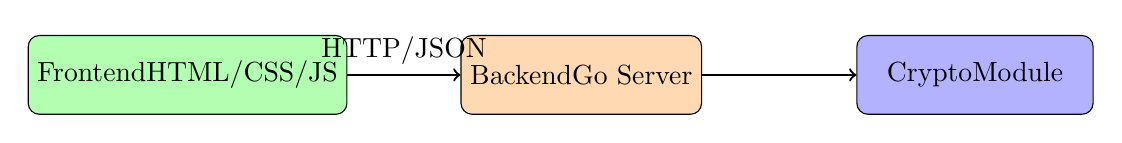
\begin{tikzpicture}[
    node distance=2cm,
    box/.style={draw, rectangle, rounded corners, minimum width=3cm, minimum height=1cm}
]
    \node[box, fill=green!30] (frontend) {Frontend\\HTML/CSS/JS};
    \node[box, fill=orange!30, right of=frontend, xshift=3cm] (backend) {Backend\\Go Server};
    \node[box, fill=blue!30, right of=backend, xshift=3cm] (crypto) {Crypto\\Module};

    \draw[->, thick] (frontend) -- node[above] {HTTP/JSON} (backend);
    \draw[->, thick] (backend) -- (crypto);
\end{tikzpicture}
\caption{Arhitectura aplicației}
\end{figure}

\subsection{Tehnologii Utilizate}

\begin{itemize}
    \item \textbf{Backend}: Go (Golang) 1.21+
        \begin{itemize}
            \item \texttt{crypto/rand} - generare numere aleatoare
            \item \texttt{crypto/aes} - implementare AES
            \item \texttt{crypto/sha256} - funcție hash
            \item \texttt{net/http} - server HTTP
            \item \texttt{encoding/json} - serializare JSON
        \end{itemize}
    \item \textbf{Frontend}: HTML5, CSS3, JavaScript (ES6+)
        \begin{itemize}
            \item Web Crypto API pentru hashing client-side
            \item Fetch API pentru comunicare cu backend
            \item CSS Grid/Flexbox pentru layout
        \end{itemize}
    \item \textbf{Documentație}: LaTeX
        \begin{itemize}
            \item Beamer pentru prezentare
            \item Article pentru raport
        \end{itemize}
\end{itemize}

\subsection{Structura Proiectului}

\begin{verbatim}
OTP-Project/
├── backend/
│   └── main.go          # Server Go + API endpoints
├── frontend/
│   ├── index.html       # Pagina principală
│   ├── styles.css       # Stiluri CSS
│   └── app.js           # Logica JavaScript
├── docs/
│   ├── presentation/
│   │   └── presentation.tex
│   └── report/
│       └── project_report.tex
└── README.md
\end{verbatim}

\subsection{API Endpoints}

\begin{table}[H]
\centering
\caption{Endpoint-uri API REST}
\begin{tabular}{|l|l|p{6cm}|}
\hline
\textbf{Endpoint} & \textbf{Metodă} & \textbf{Descriere} \\
\hline
/api/otp & POST & Criptare/Decriptare OTP \\
/api/caesar & POST & Cifrul Caesar \\
/api/vigenere & POST & Cifrul Vigenère \\
/api/aes & POST & Criptare AES-256 CBC \\
/api/hash & POST & Hash SHA-256 \\
/api/xor-analysis & POST & Demonstrație key reuse \\
\hline
\end{tabular}
\end{table}

\subsection{Rularea Aplicației}

\begin{lstlisting}[language=bash, caption=Instrucțiuni de rulare]
# Navigare in directorul backend
cd backend

# Rulare server
go run main.go

# Accesare in browser
# http://localhost:8080
\end{lstlisting}

% ============================================================
\section{Concluzii}
% ============================================================

\subsection{Rezultate}

Acest proiect a realizat:

\begin{enumerate}
    \item Implementarea funcțională a algoritmului One-Time Pad
    \item Demonstrarea practică a securității perfecte și a vulnerabilităților
    \item Comparație educativă între cifruri clasice și moderne
    \item Aplicație web interactivă pentru demonstrații
    \item Documentație completă în format LaTeX
\end{enumerate}

\subsection{Comparație Finală}

\begin{table}[H]
\centering
\caption{Comparație între algoritmii implementați}
\begin{tabular}{|l|c|c|c|c|}
\hline
\textbf{Algoritm} & \textbf{Securitate} & \textbf{Practică} & \textbf{Viteză} & \textbf{Utilizare} \\
\hline
OTP & Perfectă & Limitată & Foarte rapidă & Militar/Special \\
Caesar & Foarte slabă & Nu & Instantaneu & Educațional \\
Vigenère & Slabă & Nu & Rapidă & Educațional \\
AES-256 & Foarte puternică & Da & Rapidă & Standard \\
SHA-256 & Puternică & Da & Rapidă & Integritate \\
\hline
\end{tabular}
\end{table}

\subsection{Recomandări Practice}

\begin{enumerate}
    \item \textbf{Nu implementați propriii algoritmi criptografici} - folosiți biblioteci testate și auditate
    \item \textbf{Folosiți algoritmi moderni}: AES-256-GCM, ChaCha20-Poly1305, SHA-256/SHA-3
    \item \textbf{Generare securizată de chei}: folosiți CSPRNG (\texttt{crypto/rand} în Go)
    \item \textbf{Nu reutilizați cheile} sau IV-urile
    \item \textbf{Folosiți moduri autentificate}: GCM, Poly1305
    \item \textbf{Protejați cheile}: HSM, key derivation functions (Argon2, PBKDF2)
\end{enumerate}

\subsection{Principiul de Aur}

\begin{quote}
    \textit{"Don't roll your own crypto"} - Bruce Schneier
\end{quote}

Securitatea criptografică depinde de implementare corectă și testare riguroasă. Este întotdeauna preferabil să folosiți biblioteci și algoritmi bine stabiliți decât să creați soluții proprii.

% ============================================================
\section*{Bibliografie}
% ============================================================

\begin{enumerate}
    \item Shannon, C. E. (1949). "Communication Theory of Secrecy Systems". Bell System Technical Journal, 28(4), 656-715.
    \item Schneier, B. (2015). "Applied Cryptography: Protocols, Algorithms and Source Code in C" (20th Anniversary Edition). Wiley.
    \item Ferguson, N., Schneier, B., Kohno, T. (2010). "Cryptography Engineering: Design Principles and Practical Applications". Wiley.
    \item NIST FIPS 197. (2001). "Advanced Encryption Standard (AES)".
    \item NIST FIPS 180-4. (2015). "Secure Hash Standard (SHS)".
    \item Menezes, A. J., van Oorschot, P. C., Vanstone, S. A. (1996). "Handbook of Applied Cryptography". CRC Press.
    \item Go Crypto Package Documentation: \url{https://pkg.go.dev/crypto}
\end{enumerate}

\end{document}
